\documentclass[aspectratio=169,11pt]{beamer}

\usetheme{Singapore}
\usepackage[utf8]{inputenc}
\usepackage{amsmath}
\usepackage{amsfonts}
\usepackage{amssymb}
\usepackage{graphicx}
\usepackage{hyperref}

% Setup the bibliography
\usepackage[style=authortitle,backend=bibtex]{biblatex}
\addbibresource{bibliography.bib}
\setbeamertemplate{bibliography item}[text]
\setbeamerfont{footnote}{size=\tiny}

% Allow footnotes with no number
\newcommand\blfootnote[1]{%
  \begingroup
  \renewcommand\thefootnote{}\footnote{#1}%
  \addtocounter{footnote}{-1}%
  \endgroup
}

% Allow section title slides
\AtBeginSection[]{
  \begin{frame}
  \vfill
  \centering
  \begin{beamercolorbox}[sep=8pt,center,shadow=true,rounded=true]{title}
    \usebeamerfont{title}\insertsectionhead\par%
  \end{beamercolorbox}
  \vfill
  \end{frame}
}

\author{Dr Stephen Pederson}
\title{Lecture 2: Early Transcriptomic Strategies}
\subtitle{BIOINF3005/7160: Transcriptomics Applications}
%\setbeamercovered{transparent} 
\setbeamertemplate{navigation symbols}{} 
\logo{
	
\includegraphics[scale=0.3]{figures/UoA_logo_col_vert.png} 
} 
\institute{Bioinformatics Hub, \\The University of Adelaide} 
\date{March 16th, 2020} 
\subject{BIOINF3005/7160: Transcriptomics Applications} 


\begin{document}

\begin{frame}
\titlepage
\end{frame}

\begin{frame}
\footnotesize
\tableofcontents
\end{frame}

\section{Overview}

\linespread{1.4}

\begin{frame}{The Motivation}

	\begin{itemize}
		\item The transcriptome is a highly dynamic set of molecules
		\item Small changes can potentially have significant ramifications
		\begin{itemize}
			\item e.g. a ``Master Regulator" can determine cellular fate
		\end{itemize}
		\item RNA molecules are small
		\begin{itemize}
			\item How do we find what's in our sample?
			\item How do we quantify RNA?
			\item And how do we compare one or more groups?
		\end{itemize}
	\end{itemize}

\end{frame}

\begin{frame}{Technological Developments}

	\begin{itemize}
		\item Technological developments are constant
		\item Technologies are often transient
		\item Key technologies are:
		\begin{enumerate}
			\item Real Time Polymerase Chain Reaction (RT-PCR)
			\item Expressed Sequence Tags (EST)
			\item Serial/Cap Analysis of Gene Expression (SAGE/CAGE)
			\item Microarray technologies
			\item Sequencing technologies
		\end{enumerate}
		\item Analytic methodologies \textit{often lag technologies}
	\end{itemize}

\end{frame}

\begin{frame}{A Simplified History}

	\begin{center}
	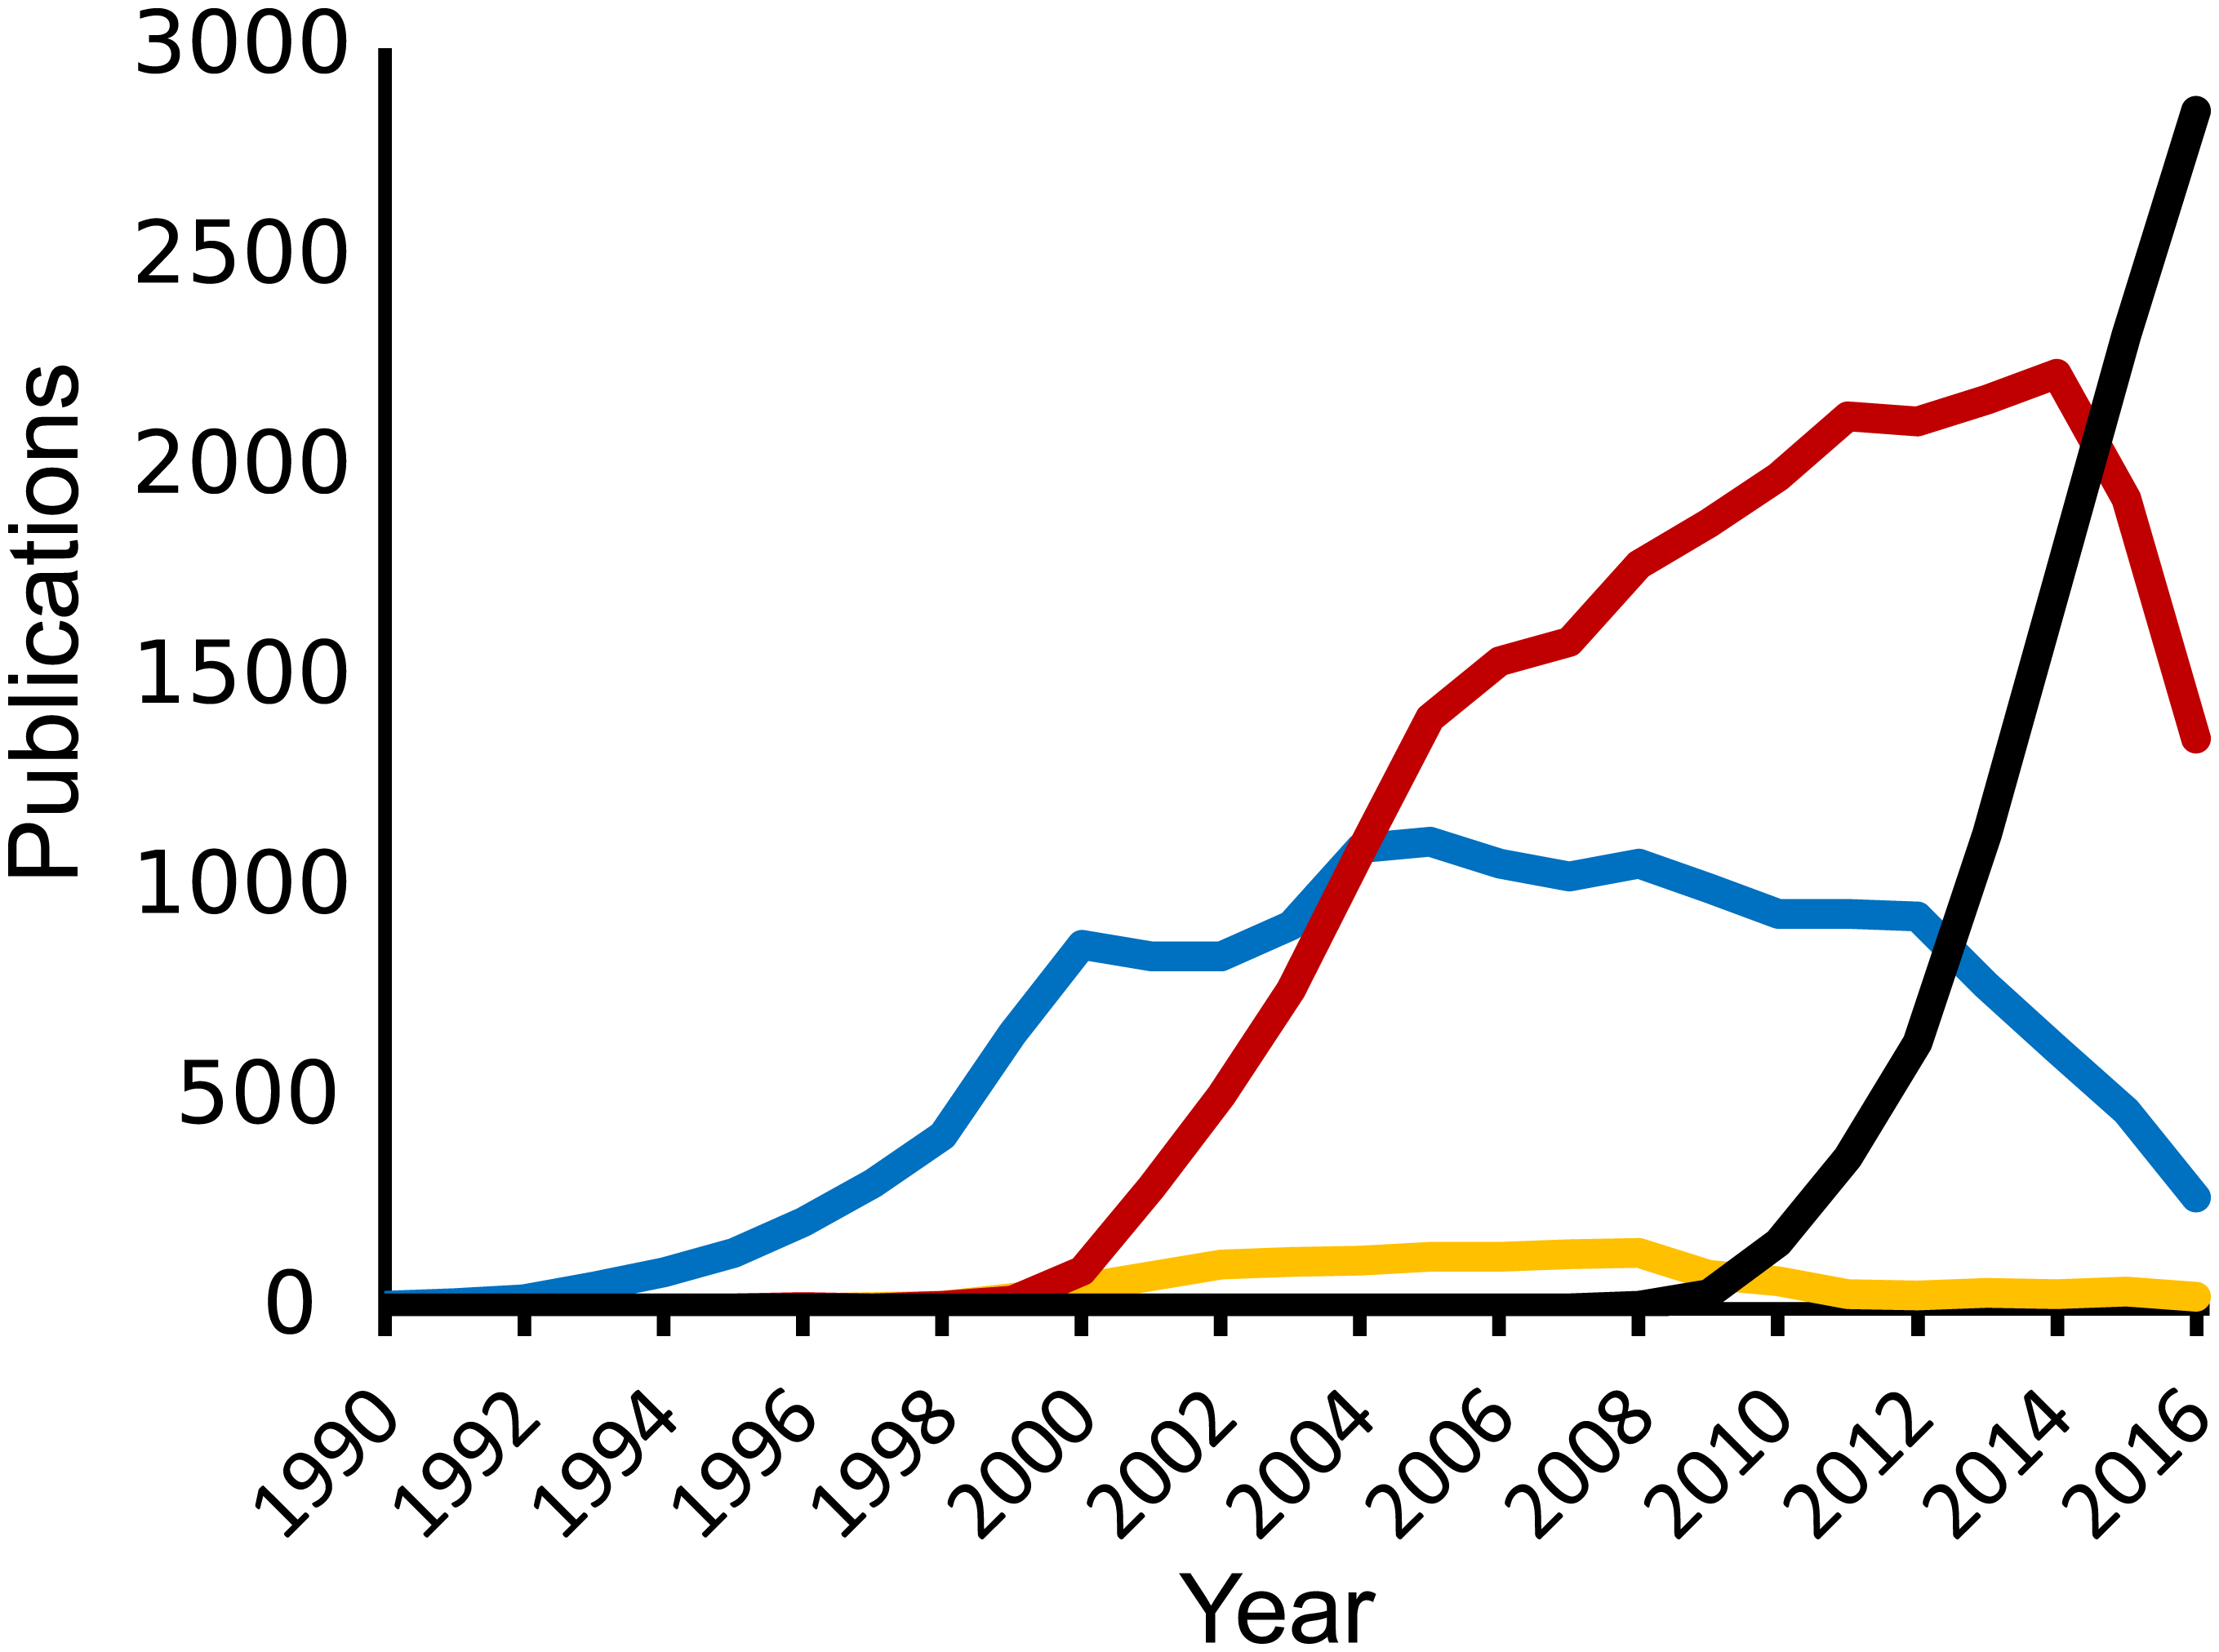
\includegraphics[scale=0.5]{figures/timeTrends.png}		
	~\\
	\textcolor[rgb]{0.1,0.4,0.7}{EST (blue)};
	\textcolor[rgb]{0.85,0.65,0.15}{SAGE / CAGE (yellow)};
	\textcolor[rgb]{0.7,0,0.2}{Microarrays (red)};  
	RNA Seq (black) \footfullcite{2017transcriptomictech}
	\end{center}
 

\end{frame}

\section{Measuring Single Genes}

%\subsection{Northern Blot}

\begin{frame}{The Northern Blot}

	\begin{itemize}
		\item One of the earliest strategies\footfullcite{1977NorthernBlot}
		\item Developed as an extension of the Southern Blot\footfullcite{pmid1195397} (DNA)
		\item Gel Electrophoresis-based strategy
		\begin{itemize}
			\item Based on size differentiation and probe sequences
		\end{itemize}
	\end{itemize}

\end{frame}

\begin{frame}{The Northern Blot}

	\begin{itemize}
		\item RNA is extracted then denatured
		\item RNA is size separated using Gel Electrophoresis
		\item RNA is transferred to a ``blotting membrane"
		\item Treat the membrane with a labelled probe
		\begin{itemize}
			\item Probes are complementary to the ``target sequence"
			\item Probes are labelled with fluorescent dye or radioactive atoms
		\end{itemize}
	\end{itemize}

\end{frame}

\begin{frame}{The Northern Blot}

	\begin{center}
		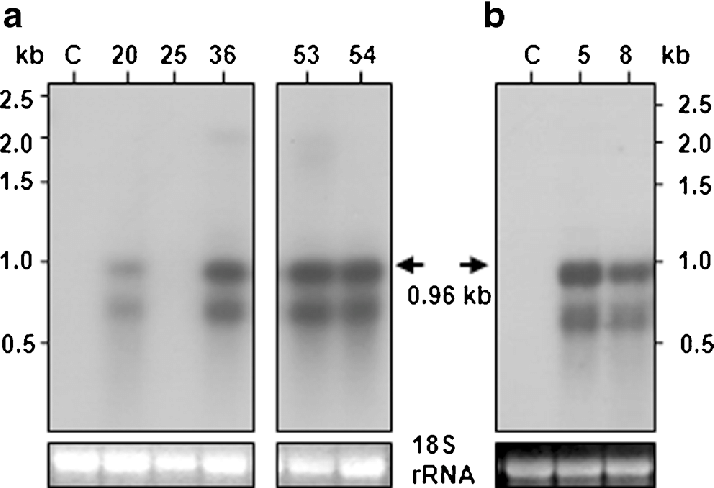
\includegraphics[scale=0.3]{figures/northern.png} 
	\end{center}

\blfootnote{Taken from \cite{pmid25648206}}	

\end{frame}

\begin{frame}{The Northern Blot}
	\begin{itemize}
		\item Prominent usage \textit{before} genomes were sequenced
		\item Can possibly detect different isoforms
		\item Crude quantitation using Densitometric Analysis
		\begin{itemize}
			\item What limitations might this have?
			% \item Not accurate for low abundance
			% \item Very time intensive
			% \item Requires large amounts of starting material
		\end{itemize}
	\end{itemize}
\end{frame}

%\subsection{RT-PCR}

\begin{frame}{RT-qPCR}

	\begin{itemize}
		\item Reverse Transcriptase quantitative PCR
		\begin{itemize}
			\item Sometimes called: qPCR, RT-PCR
		\end{itemize}
		\item Often considered to be the ``gold standard" for quantitation
		\item Targets a \textit{specific transcribed region} via \textit{specific primers}
		\begin{itemize}
			\item Primers must be individually designed
			\item Primers often span exon-exon junctions
		\end{itemize}
	\end{itemize}

\end{frame}

\begin{frame}{RT-qPCR}

	\begin{enumerate}
		\item \textit{Reverse Transcriptase} converts RNA to cDNA
		\begin{itemize}
			\item Primers are required: Can target polyA or random
		\end{itemize}
		\item Sequence-specific primers amplify the target fragment in cycles
		\begin{itemize}
			\item Fluorescent dye is commonly incorporated during amplification
		\end{itemize}
		\item Abundance of target will grow exponentially ($\times 2$) for each amplification cycle
		\item The cycle where abundance reaches the ``limit of detection" is estimated ($C_T$)
	\end{enumerate}

\end{frame}

\begin{frame}{RT-qPCR}

	\begin{center}
	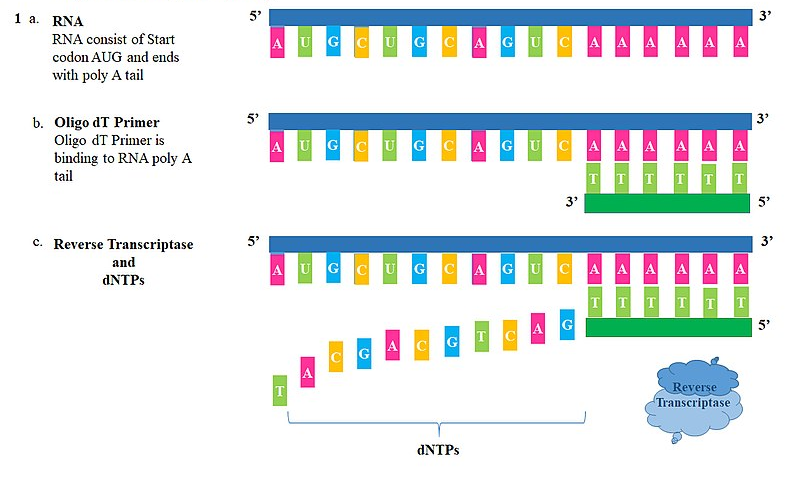
\includegraphics[scale=0.3]{figures/RTqPCR1.png} 
	\end{center}
	
	\blfootnote{Modified from \cite{By Lokeshthimmana - Own work, CC BY-SA 4.0, https://commons.wikimedia.org/w/index.php?curid=76313637}}	

\end{frame}

\begin{frame}{RT-qPCR}

	\begin{center}
	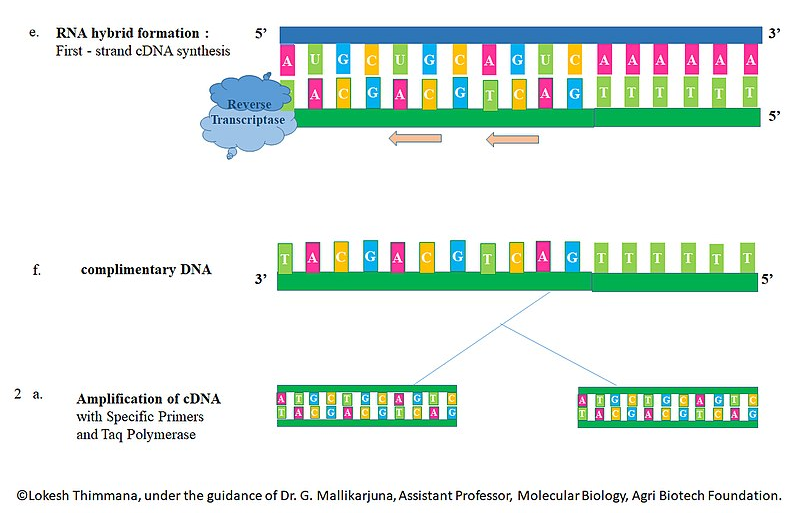
\includegraphics[scale=0.3]{figures/RTqPCR2.png} 
	\end{center}
	
	\blfootnote{Modified from \cite{By Lokeshthimmana - Own work, CC BY-SA 4.0, https://commons.wikimedia.org/w/index.php?curid=76313637}}	

\end{frame}

\begin{frame}{RT-qPCR}

	\begin{center}
		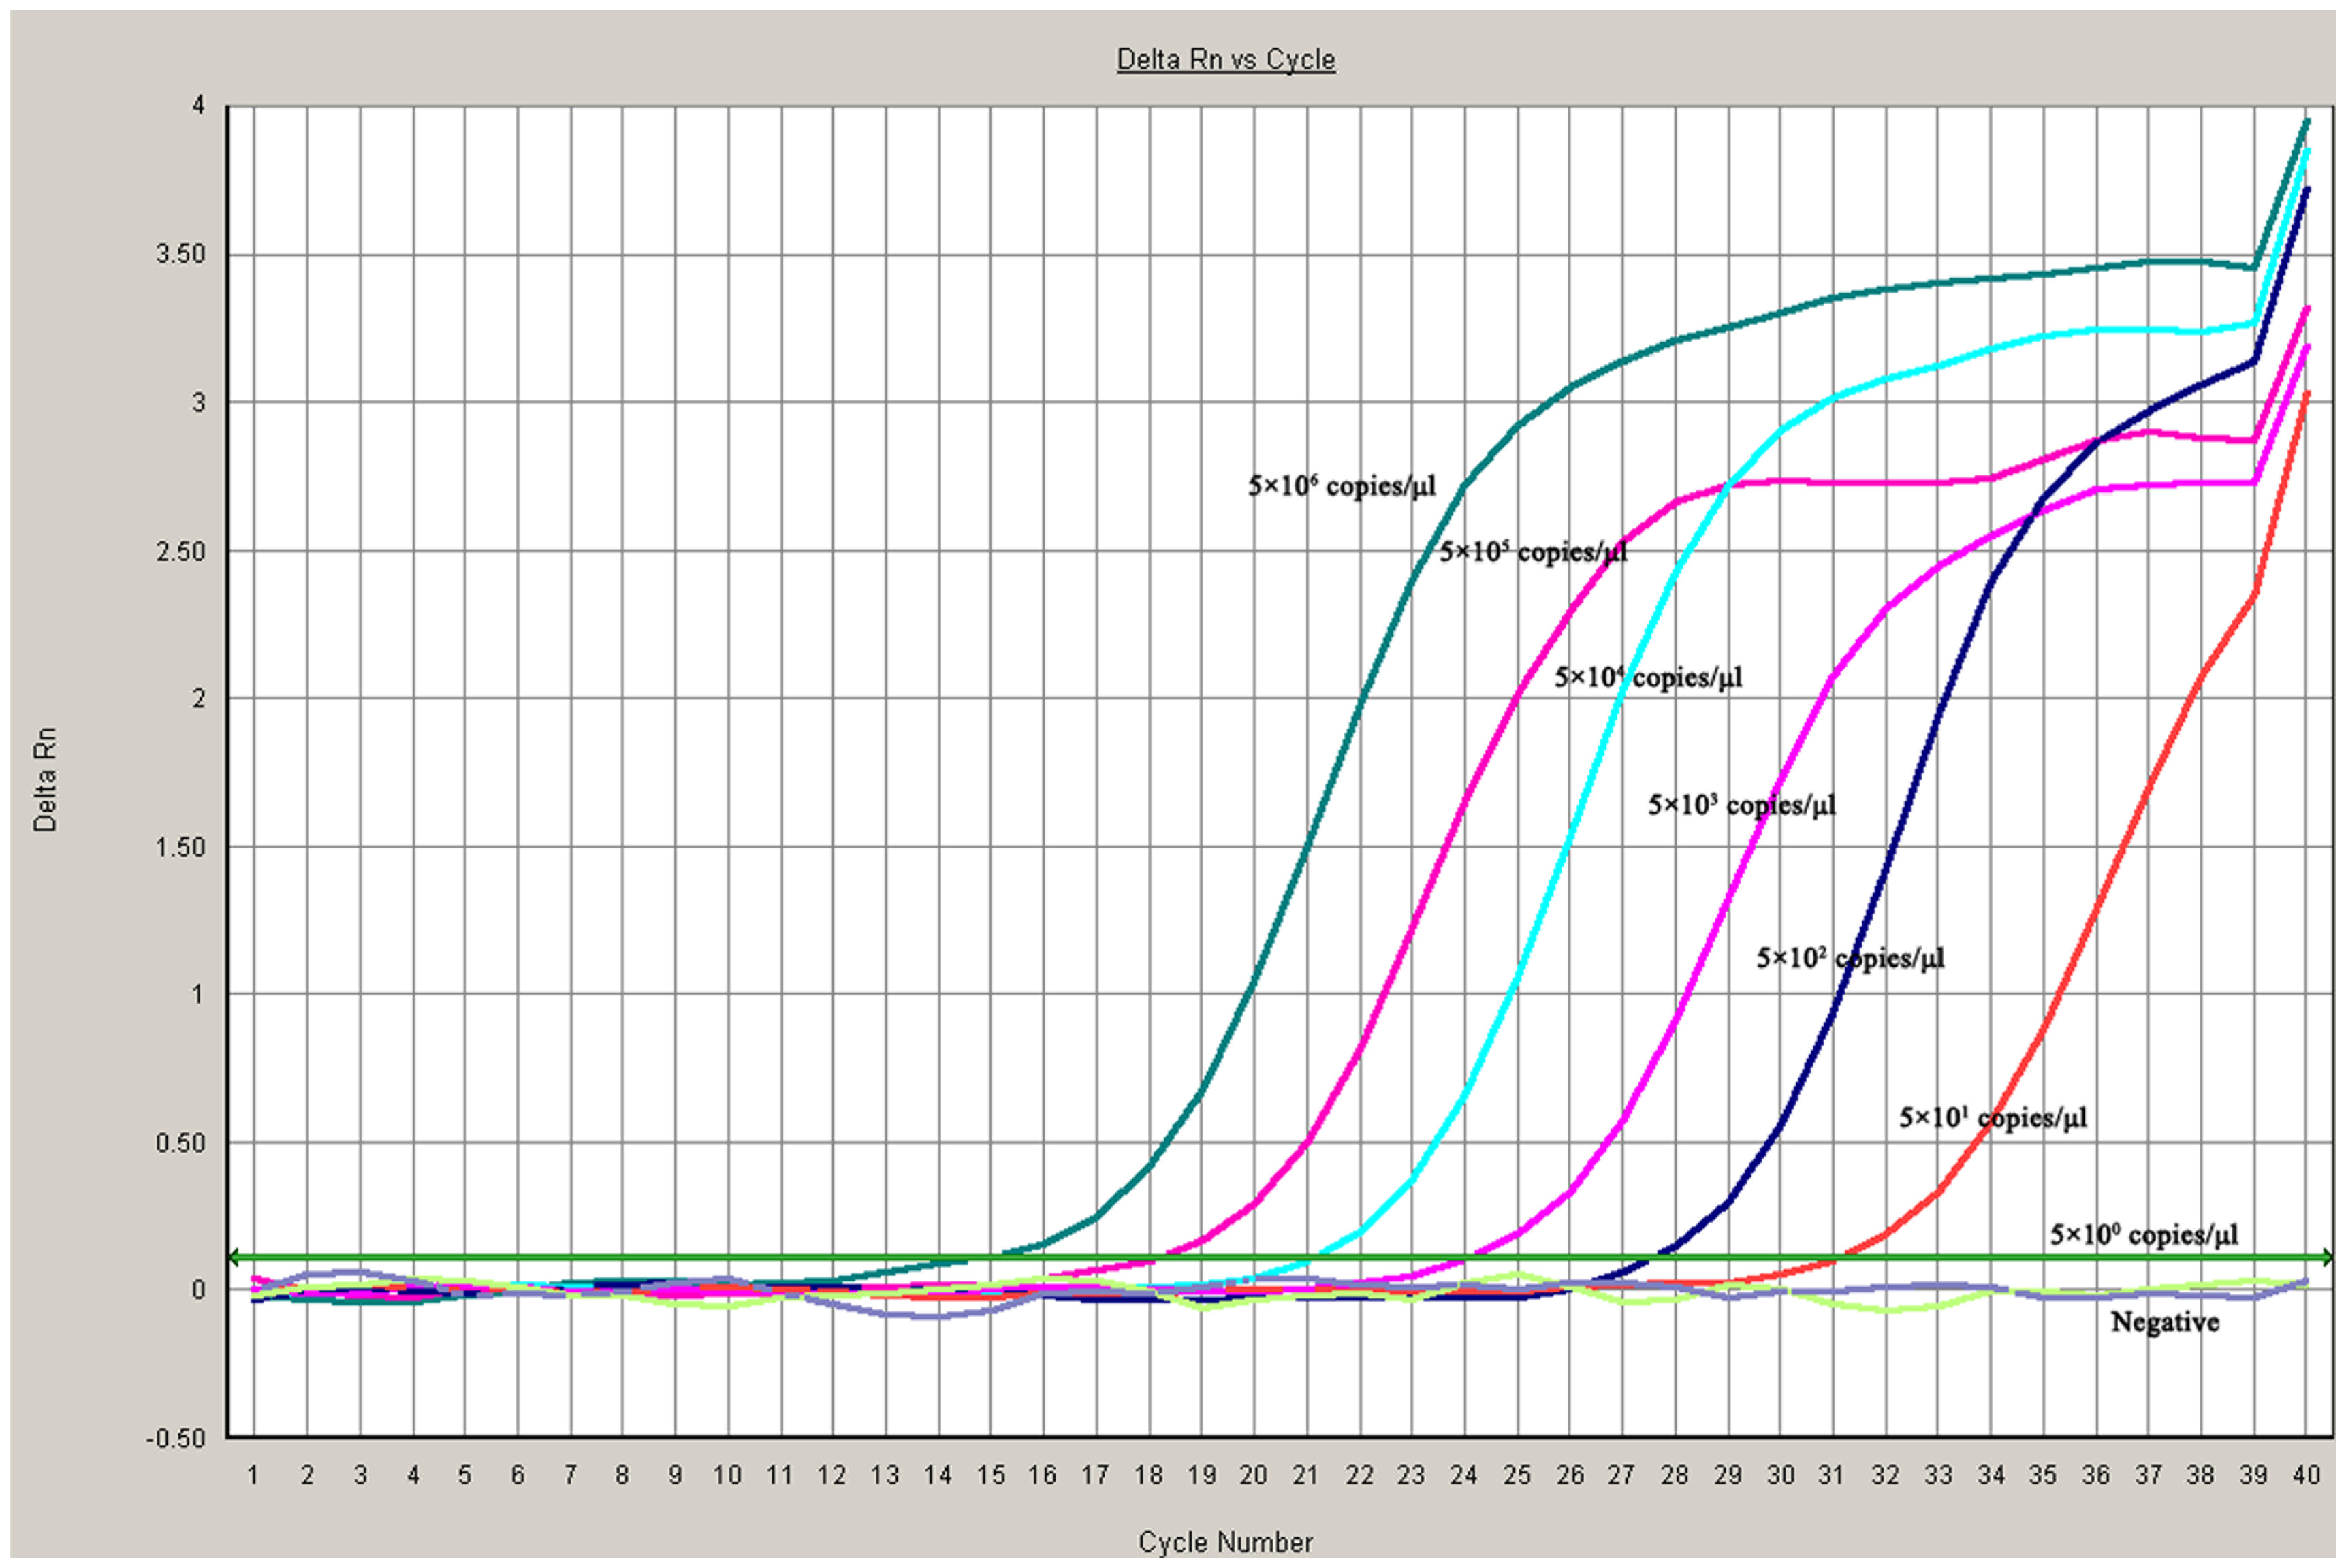
\includegraphics[scale=0.5]{figures/qPCR.png} 
		~\\
		This is a 10-fold dilution series\footfullcite{2013qPCR}
	\end{center}

\end{frame}

\begin{frame}{RT-qPCR}

	\begin{itemize}
		\item Can be used with a standard curve and dilution series to estimate absolute quantity of an RNA \textit{within a sample}
		\item Can be used to compare \textit{across samples for relative abundance}
	\end{itemize}
	\pause
	\begin{center}
		~\\
		\textit{What may be a fundamental issue when comparing across samples?}
	\end{center}


\end{frame}

\begin{frame}{Normalisation}

	\begin{itemize}
		\item There may be pipetting and other technical differences between samples
		\begin{itemize}
			\item These are \textbf{non-biological} in origin
		\end{itemize}
		\item To correct for these we can \textbf{normalise} our data
		\item In RT-qPCR this is often done using ``housekeeper" genes
		\begin{itemize}
			\item We choose genes which \textit{should not} change between samples/groups
			\item These are commonly structural genes such as \textit{ACTN$\beta$} or \textit{GAPDH}
		\end{itemize}
	\end{itemize}

\end{frame}

\begin{frame}{Estimating Change In Expression}

	\begin{itemize}
		\item Relative abundances are often referred to as fold-change (FC)
		\begin{itemize}
			\item Down regulation is squeezed between 0 and 1
			\item Up regulation ranges from 1 to $\infty$
		\end{itemize}
		
		\item We often use $\log_2$ fold-change to get a better scale, e.g. 
		\begin{itemize}
			\item A 2-fold increase in abundance: $\log_2 2^1=1$
			\item A 2-fold decrease in abundance: $\log_2 \frac{1}{2}= \log_2 2^{-1} = -1$
			\item No change in abundance $\log_2 1 = \log_2 2^0 = 0$
		\end{itemize}		 
		\item This is often abbreviated as \textit{logFC}
	\end{itemize}

\end{frame}

\begin{frame}{Estimating Change In Expression}

	\begin{itemize}
		\item For \textit{RT-qPCR} the estimate of \textit{logFC} is known as $\Delta\Delta C_T$
		\item To calculate this, we calculate \textbf{two} changes in $C_T$
		\begin{enumerate}
			\item $\Delta C_T$ relative to the housekeeper(s)
			\item $\Delta \Delta C_T$ across samples for our gene/fragment of interest 
		\end{enumerate}
		\item The first step corrects for technical errors
		\item The second step estimates our true change in abundance
	\end{itemize}

\end{frame}

\begin{frame}{Estimating Change In Expression}

	Within each sample

	\begin{align*}
	\Delta C_T = C_{t[\text{gene}]} - C_{t[\text{HK}]}
	\end{align*}
	
	Across samples/groups
	
	\begin{align*}
	\Delta \Delta C_T = - (\Delta C_{T[\text{group1}]} - \Delta C_{T[\text{group2}]})
	\end{align*}
	
	This formulation assumes \textit{equal amplification efficiency} for all primers/genes (i.e. \textit{Efficiency} $= 2$)

\end{frame}

\begin{frame}{Estimating Change In Expression}

	\begin{itemize}
		\item Housekeeper genes must be matched to the ``gene of interest" \textbf{within each sample} and \textbf{within each qPCR reaction}
		\item Choosing $>1$ housekeeper gene is advised
		\item Measurements are often taken in triplicate/quadruplicate for each sample (reactions sometimes fail)
	\end{itemize}
	
	~\\
	\textit{Both Northern blots and RT-qPCR use targeted primers, but in very different ways}

\end{frame}

\section{Measuring Multiple Genes}

%\subsection{EST}

\begin{frame}{Expressed Sequence Tags}

\end{frame}

\subsection{CAGE}


\end{document}